\documentclass[a4paper,11pt]{article}
\pdfoutput=1 % if your are submitting a pdflatex (i.e. if you have
             % images in pdf, png or jpg format)

\usepackage{jheppub} % for details on the use of the package, please
                     % see the JHEP-author-manual

\usepackage[T1]{fontenc} % if needed
\usepackage{amsmath}
\usepackage{graphicx}
\usepackage[colorinlistoftodos]{todonotes}
%\usepackage[colorlinks=true, allcolors=blue]{hyperref}

\newcommand{\CH}[1] {\textbf{\textcolor{blue}{CH - #1}}}
\newcommand{\MS}[1] {\textbf{\textcolor{purple}{MS - #1}}}
\newcommand{\MLM}[1] {\textbf{\textcolor{green}{MLM - #1}}}
\newcommand{\TR}[1] {\textbf{\textcolor{red}{TR - #1}}}
\newcommand{\DA}[1] {\textbf{\textcolor{orange}{DJ - #1}}}


\newcommand{\Zp}{\ensuremath{Z^{\prime}}}
\newcommand{\ZpSSM}{\ensuremath{Z^{\prime}_{\mathrm{SSM}}}}
\newcommand{\Z}{\ensuremath{Z}}
\newcommand*{\Zptata}{\ensuremath{Z^{\prime}\rightarrow \tau\tau}}
\newcommand*{\Zpee}{\ensuremath{Z^{\prime}\rightarrow \text{e e}}}
\newcommand*{\Zpmumu}{\ensuremath{Z^{\prime}\rightarrow \mu\mu}}
\newcommand*{\Zpll}{\ensuremath{Z^{\prime}\rightarrow \ell\ell}}
\newcommand*{\Zptt}{\ensuremath{Z^{\prime} \rightarrow \ttbar}}
\newcommand{\ptSub}[1]{\ensuremath{p_{\text{T} #1}}}
\newcommand{\ptSup}[1]{\ensuremath{p_{\text{T}}^{#1}}}
\newcommand{\pt}{\ensuremath{p_{\text{T}}}}
\newcommand{\ptEl}{\ensuremath{p_{\text{T}}^{e}}}
\newcommand{\ptMu}{\ensuremath{p_{\text{T}}^{\mu{}}}}
\newcommand{\ptZp}{\ensuremath{p_{\text{T}}^{\ensuremath{Z^{\prime}}}}}
\newcommand{\mZp}{\ensuremath{M_{\ensuremath{Z^{\prime}}}}}
\newcommand{\mSD}{\ensuremath{m_{\ensuremath{SD}}}}
\newcommand{\mll}{\ensuremath{M_{\ensuremath{ll}}}}
\newcommand*{\hht}{\ensuremath{H_{\ensuremath{T}}}}
\newcommand*{\met}{\ensuremath{E_{T}^{\rm{miss}}}}
\newcommand*{\intlumifcc}{\ensuremath{\mathcal{L}=30\text{ ab}^{-1}}}
\newcommand*{\intlumihelhc}{\ensuremath{\mathcal{L}=15\text{ ab}^{-1}}}
\newcommand*{\qjj}{\ensuremath{Q^{*} \rightarrow jj}}
\newcommand*{\rsg}{\ensuremath{G_{RS} \rightarrow WW}}
\newcommand*{\vj}{\ensuremath{\text{V + jets}}}
\newcommand*{\metvec}{\vec{\pt}^{\textrm{miss}}}

\newcommand*{\ee}{\ensuremath{e^{+}e^{-}}}
\newcommand*{\mumu}{\ensuremath{\mu^{+}\mu^{-}}}
\newcommand*{\tautau}{\ensuremath{\tau^{+}\tau^{-}}}
\newcommand*{\ellell}{\ensuremath{\ell^{+}\ell^{-}}}
\newcommand*{\ttbar}{\ensuremath{t\bar{t}}}
\newcommand*{\bbbar}{\ensuremath{b\bar{b}}}
\newcommand*{\ww}{\ensuremath{W^{+}W^{-}}}
\newcommand*{\jj}{\ensuremath{jj}}


\newcommand{\amc}{{\sc MadGraph5\textunderscore}a{\sc MC@NLO}}
\newcommand{\pys}{{\sc Pythia6}}
\newcommand{\delphes}{{\sc Delphes3}}

\def\ifb{\mbox{fb$^{-1}$}}%  Inverse femtobarns.
\def\afb{\mbox{ab$^{-1}$}}%  Inverse atobarns.

\def\TeV{\ifmmode {\mathrm{\ Te\kern -0.1em V}}\else
                   \textrm{Te\kern -0.1em V}\fi}%
\def\GeV{\ifmmode {\mathrm{\ Ge\kern -0.1em V}}\else
                   \textrm{Ge\kern -0.1em V}\fi}%
\def\MeV{\ifmmode {\mathrm{\ Me\kern -0.1em V}}\else
                   \textrm{Me\kern -0.1em V}\fi}%
\def\keV{\ifmmode {\mathrm{\ ke\kern -0.1em V}}\else
                   \textrm{ke\kern -0.1em V}\fi}%
\def\eV{\ifmmode  {\mathrm{\ e\kern -0.1em V}}\else
                   \textrm{e\kern -0.1em V}\fi}%


\title{\boldmath Heavy resonances at energy frontier colliders}

\author[a,c]{David~Jamin}
\author[a]{\!\!, Clement~Helsens}
\author[a]{\!\!, Michelangelo~L.~Mangano}
\author[b]{\!\!, Thomas~G.~Rizzo}
\author[a]{and Michele~Selvaggi}

\affiliation[a]{CERN, CH-1211 Geneva 23, Switzerland}
\affiliation[b]{SLAC National Accelerator Laboratory 2575 Sand Hill Rd., Menlo Park, CA, 94025 USA}
\affiliation[c]{Academia Sinica, Institute of  Physics, Taipei, Taiwan}

% e-mail addresses: one for each author, in the same order as the authors
\emailAdd{first@one.univ}
\emailAdd{second@asas.edu}
\emailAdd{third@one.univ}
\emailAdd{fourth@one.univ}


\abstract{This paper explores the physics reach of the proton-proton Future Circular Collider (FCC-hh) and High Energy LHC (HE-LHC) for searches of new particles decaying to two high energetic leptons, jets (non-tops), tops and W/Z boson. We discuss the expected exclusion limits and discovery potential for benchmark models predicting new massive particles that result in resonant structures in the invariant mass spectrum. This document also includes a detailed study on the discrimination potential of a $\Zp$ at HE-LHC in case of discovery at the end of High-Luminosity LHC (HL-LHC).}

\begin{document}
\maketitle
\flushbottom

\section{Introduction}
\label{sec:intro}

Particle accelerators are built to answer some of the most fundamental questions about the natural world. For LHC it was guaranteed that the Standard Model (SM) Higgs boson would be found, for the next generation of machines there is no possibilities to guarantee that any new particle will be discovered. Still with much higher center of mass energies compared to LHC, there are guaranteed deliverables like the study of the Higgs and top-quark properties and exploration of electroweak symmetry breaking phenomena with unmatchable precision and sensitivity.

New machines are build to make direct discoveries, and even though we do not have any guarantee discoveries, we need to make sure that we will cover a large fraction of Beyond the SM (BSM) phase space. So the mass reach should be increased by a factor of $\sqrt{s}/14$ so 7 for $\sqrt{s}=100$, but there are issues with parton luminosities evolving with $Q^2$, as at high energy they drop a bit faster, so typically it is a factor of 5 increase. But the statistics is enhanced by several orders of magnitudes for many BSM phenomena, that the LHC could barely touch during its exploitation. It is not only that the mass reach increases by a large factor, but it is the fact that if the LHC were to see some hints of possible new physics, by increasing the energy by a factor seven, we would increase the statistics by two or even three orders of magnitude, and we can use this new machine to study with great accuracy what it is about exactly.
In addition we could have the ability to provide firm answers to questions like: is the SM dynamics all there at the TeV scale, is there a TeV scale solution to the hierarchy problem, is dark matter a thermal wimp (either we discover it as a WIMP, or we discover DM is not a WIMP and it has to be something else), was the cosmological EW phase transition 1st order, etc...

Concerning the topic of this paper, the discovery potential of new resonances not predicted by the SM makes Future Circular Colliders (FCC) to be the only  place to search for such heavy particles, compared to the current LHC and coming HL-LHC.
In the framework of FCC it is also extremely relevant to discuss the main limitations of the detector to identify high energetic top-quarks or W/Z bosons. Indeed 100\,TeV proton-proton collisions will produce a very large amount of multi-TeV's bosons or top, thus the design of the detector needs detailed optimisations in order to achieve the required physics goals. The capabilities of such a detector should include the capabilities of measuring multi-TeV leptons, top-quarks and bosons, and will be discussed in this paper.

This document presents the expectations of some of the most relevant BSM scenarios and the considered models are detailed in the section~\ref{sec:physmodel}.
The sample production, detector parametrisation, analysis statistical methods and other analysis techniques developed are presented in the section~\ref{sec:fccworkflow}.
The leptonic resonances (ee, $\mu\mu$, $\tau\tau$) and the hadronic resonances (WW, $t\bar{t}$ and jj) analyses are detailed in sections~\ref{subsec:lepreso} and~\ref{subsec:hadreso} respectively.
The analyses strategy started from optimisation at FCC-hh, but the results have also been extracted in the case of the HE-LHC scenario (section~\ref{sec:ana27tev}).
Finally, a study of model discrimination at HE-LHC in case of discovery at the end of HL-HLC is presented in section~\ref{sec:modeldiscri}.

\section{Simulation setup}
\label{sec:simulation}

%%%%%%%%%%%%%%%%%%%%%%%%%%%%%%%%%%%%%%%%%%%%%%%%%%%%%
\subsection{Monte-Carlo production}
\label{subsec:mcprod}

% /eos/experiment/fcc/helhc/utils/delphescards/helhc_v01/card.tcl
% /eos/experiment/fcc/hh/utils/delphescards/fcc_v02/muonMomentumResolutionVsP.tcl
Monte Carlo~(MC) simulated event samples were used to simulate the response of the detector to signal and backgrounds. Signals are generated with {\scshape Pythia}~8.230~\cite{Sjostrand:2014zea} using the leading order cross-section from the generator.
All lepton flavour decays of the $\ZpSSM$ are generated assuming universality of the couplings.\CH{do we need this here? That's too little information, we need a more complete description of all the various processes.}
The SM backgrounds are Drell-Yan, di-jet (QCD), top pairs (\ttbar), $VV$ and \vj\ where $V=W/Z$,  were generated using \amc~\cite{Alwall:2014hca} at leading order only. A k-factor of 2 is applied to all the background processes to account for higher order corrections.
Independent samples have been generated for the training of object tagger described in section~\ref{subsec:mvatagger}.

%{\scshape Pythia} independent samples have been produced for Multi-Variate taggers training (section~\ref{subsec:mvatagger}). QCD has been produced to avoid useless events thanks to a filtering chosen to ensure to have consistent leading jet $\pT$ as the signals considered (pTHatMin = 2500, bias2Selection = on, bias2SelectionPow = 6).\newline
%Tables~\ref{tab:MCtable_bkgd} and ~\ref{tab:MCtable_sig} are summarising all the background and signal samples produced for the various analysis presented in this document.

%\begin{table}[!htb]\centering
%\begin{tabular}{|c|c|c|c|}
%\hline
%\hline
%process & Ngen & generator & k-factor \\
%\hline
%pp\_$ee$\_5f\_HT & $\sim$5M & $mg+p8$ & 2 \\
%pp\_$\mu\mu$\_5f\_HT & $\sim$5M & $mg+p8$ & 2 \\
%pp\_$\tau\tau$\_5f\_HT & $\sim$5M & $mg+p8$ & 2 \\
%pp\_$jj$\_5f\_HT ($j$ = $u$, $d$, $c$, $s$ or $b$) & $\sim$5M & $mg+p8$ & 2 \\
%pp\_$tt$\_5f\_HT & $\sim$5M & $mg+p8$ & 2 \\
%pp\_$Vj$\_5f\_HT ($V$ = $W$ or $Z$ and $j$ = $u$, $d$, $c$, $s$ or $b$) & $\sim$5M & $mg+p8$ & 2 \\
%pp\_$VV$\_5f\_HT ($V$ = $W$ or $Z$) & $\sim$5M & $mg+p8$ & 2 \\
%\hline
%\hline
%\end{tabular}
%\caption{Summary of generated background samples. The following HT (scalar sum of all visible paticles momentum at generator level) binnings have been used : [500, 1000], [1000, 2000], [2000, 5000], [5000, 10000], [10000, 27000], and [27000, 100000] GeV. 5f stands for flavour quaks : u, d, c ,s  and b.}
%\label{tab:MCtable_bkgd}
%\end{table}

%\begin{table}[!htb]\centering
%\begin{tabular}{|c|c|c|c|}
%\hline
%\hline
%process & Ngen & generator & k-factor \\
%\hline
%pp\_$Z'_{SSM}$\_$ll$ ($l$ = $e$, $\mu$ or $\tau$) & \multirow{2}{*}{$\sim$1M} & \multirow{2}{*}{$p8$} & \multirow{2}{*}{1} \\
%mass : \{2,4,5,6,8,10,12,14,15,16,18,20,25,30,35,40,45,50\} TeV & & & \\
%\hline
%pp\_$Z'_{flavano}$\_$\mu\mu$\_5f & \multirow{2}{*}{$\sim$1M} & \multirow{2}{*}{$mg+p8$} & \multirow{2}{*}{1} \\
%mass : \{4,6,8,10,12,14,15,16,18,20,25,30,35,40,45\} TeV & & & \\
%\hline
%pp\_$LQ$\_$\mu\mu$\_5f & \multirow{2}{*}{$\sim$1M} & \multirow{2}{*}{$mg+p8$} & \multirow{2}{*}{1} \\
%mass : \{4,6,8,10,12,14,16,18,20,22,24,26,28,30,32,34,36,38,40\} TeV & & & \\
%\hline
%pp\_$Z'_{TC2}$\_$tt$ & \multirow{2}{*}{$\sim$1M} & \multirow{2}{*}{$p8$} & \multirow{2}{*}{1} \\
%mass : \{2,5,10,15,20,25,30,35\} TeV & & & \\
%\hline
%pp\_$RSG$\_$WW$ & \multirow{2}{*}{$\sim$1M} & \multirow{2}{*}{$p8$} & \multirow{2}{*}{1} \\
%mass : \{2,5,10,15,20,25,30,35\} TeV & & & \\
%\hline
%pp\_$Q^*$\_$qq$ ($q$ = $u$, $d$, $c$, $s$, $b$ or $t$) & \multirow{2}{*}{$\sim$0.6M} & \multirow{2}{*}{$p8$} & \multirow{2}{*}{1} \\
%mass : \{15,20,25,30,35,40,45,50\} TeV & & & \\
%\hline
%pp\_$Z'_{SSM}$\_$jj$ ($j$ = $u$, $d$, $c$, $s$ or $b$) & \multirow{2}{*}{$\sim$1.2M} & \multirow{2}{*}{$p8$} & \multirow{2}{*}{1} \\
%mass : \{10,15,20,25,30,35,40,45,50\} TeV & & & \\
%\hline
%\hline
%\end{tabular}
%\caption{Summary of generated signal samples.}
%\label{tab:MCtable_sig}
%\end{table}

%%%%%%%%%%%%%%%%%%%%%%%%%%%%%%%%%%%%%%%%%%%%%%%%%%%%%%%%%%%%%%%%%%%%%%%%%%%%%%%%%%%%%%%%%%%%
\subsection{Detector parameterizations}
\label{subsec:detparam}

As part of the FCC study group, the \delphes\ software package~\cite{deFavereau:2013fsa} is used to emulate the response a detector.
For the FCC-hh and HE-LHC the basic performances can be summarised as follow: The muon momentum resolution is assumed to be $\sigma(p)/p \approx 6\%~(10\%)$ at $\pt= 20~(5)$ TeV and $|\eta| \approx 0.$ for FCC-hh (HE-LHC) scenario.
\CH{maybe we need a table to compare basic performances of FCC and HE-LHC like~\ref{tab:delphes_comp}}.

\begin{table}[!htb]\centering
\begin{tabular}{|c|c|c|}
\hline
 & FCC-hh & HE-LHC \\
 muon & & \\
\hline
 electron  & & \\
\hline
 tau  & & \\
\hline
 jets & & \\
\hline
  b-jets  & & \\
\hline
\end{tabular}
\caption{Comparison of basic detector performances.}
\label{tab:delphes_comp}
\end{table}


%%%%%%%%%%%%%%%%%%%%%%%%%%%%%%%%%%%%%%%%%%%%%%%%%%%%%
\subsection{Multi-Variate object tagging}
\label{subsec:mvatagger}

% from physics paper
An important ingredient of the \Zptt\ and \rsg\ searches is the identification of heavy boosted top quarks and $W$ bosons. Two object level taggers using Boosted Decision Trees (BDT) were developed to discriminate $W$ and top jets against the light jets treated as background. Jets containing leptons, for example from sem-leptonic b-decays, are removed from the training.
%The BDT parameters used are the following : NTrees=600, MaxDepth=4, AdaBoost, AdaBoostBeta=0.15, SeparationType=GiniIndex, nCuts=100, PruneMethod=NoPruning.
%The input variables are defined to be the same as the ones used to perform cut-based associated analysis (\Zptt\ and \rsg\ in section~\ref{subsec:hadreso}) and the idea is to fully exploit these informations thanks to the BDT.
The input variables used to train the BDT, ordered by training weight, can be found in table~\ref{tab:TMVA_summary}.
Top and $W$ taggers were optimised using jets with a transverse boost of $\pt=$10 TeV. At these extreme energies, $W$ and top jets have a characteristic angular size $R=0.01-0.02$, i.e smaller than the typical electromagnetic and hadronic calorimeter cells. Following the approach described in~\cite{Larkoski:2015yqa}, we exploit the superior track angular resolution and reconstruct jets from tracks only using the anti-$k_T$ algorithm with a parameter R=0.2, but also larger values are used to increase the discrimination power of the BDT. The missing neutral energy is corrected for by rescaling the track 4-momenta by the factor $\ptSub{,trk}/\ptSub{,PF}$, where $\ptSub{,trk}$ is the track Jet \pt\ and $\ptSub{,PF}$ is the Particle-Flow (PF) Jet \pt. In what follows, we will simply refer to ``track jets'' as the jet collection that includes the aforementioned rescaling.
\newline
The boosted top tagger is built from jet substructure observables: the soft-dropped jet mass~\cite{Larkoski:2014wba} (\mSD) and N-subjettiness~\cite{Thaler:2010tr} variables $\tau_{1,2,3}$ and their ratios $\tau_{2}/\tau_{1}$ ($\tau_{21}$) and $\tau_{3}/\tau_{2}$ ($\tau_{32}$). The $W$-jet tagger also uses an ``isolation-like'' variable that exploits the absence of high \pt\ final state-radiation (FSR) in the vicinity of the $W$ decay products. We call these variables $E_{F}(n,\alpha)$ and define them as:

%\begin{equation}
%E_{F}(n,\alpha) =  \frac{\sum \limits_{\frac{n-1}{5}\alpha < \Delta R(k,jet)< \frac{n}{5}\alpha} \ptSup{(k)}}{\sum \limits_{\Delta R(k,jet)< \alpha} \ptSup{(k)}}
%\end{equation}

\begin{equation}
E_{F}(n,\alpha) =  \sum \limits_{\frac{n-1}{5}\alpha < \Delta R(k,jet)< \frac{n}{5}\alpha} \ptSup{(k)} \Biggm/ \sum \limits_{\Delta R(k,jet)< \alpha} \ptSup{(k)}
\end{equation}
with $k$ running over the jet constituents and $\alpha=0.05$. We construct 5 variables $E_{F}(n,\alpha)$ with $n=[1,2,3,4,5]$ and use them as input to the BDT.
As an example, the $E_{F}(n=1,\alpha=0.05)$ observable is shown in Figures~\ref{fig:TMVA_final_result} left and~\ref{fig:TMVA_inputs_w}.
The final performance of the $W$ and top tagger is shown in Figure~\ref{fig:TMVA_final_result} (right). More $TMVA$ (Toolkit for Multivariate Data Analysis) detailed results can be found in appendix~\ref{appendix:tmva}.
The $W$ tagging performance has significantly better performance due to the use of the energy-flow variables. We choose the working points for the analyses presented later with a top and $W$ tagging efficiencies of $\epsilon_S^{\text{top}}=60\%$ and $\epsilon_S^{\text{W}}=90\%$ corresponding respectively to a background rejection of $\epsilon_B^{\text{top}}=\epsilon_B^{\text{W}}=90\%$. These working points corresponds to a cut at 0.15 on the BDT value for both taggers. The evolution of the light jet efficiency versus the $W$ and top tagging efficiencies for both taggers is shown in Figure~\ref{fig:TMVA_final_result} right.
\newline
Some extra cross-checks have been performed. First, by removing highly correlated variables, such as \CH{@David Add example}, it showed the same performances \CH{@ David, then why don't we remove the correlated variables?}.
As a second test, the BDT response has been tested for different signal masses to understand how the mass dependence could affect the analyses (Figure \ref{fig:BDT_signal_shape_comparison}). For the cut used in the analysis (BDT score greater than 0.15), the shape of the BDT is not dramatically changing the signal efficiency.% and it removes 90\% and 95\% of light jets for thad and Whad taggers respectively.

\begin{table}[!htb]\centering
\begin{tabular}{| l | c | l | c |}
\hline
  \multicolumn{2}{|c|}{$W$ tagger}  & \multicolumn{2}{c|}{top tagger} \\
  \hline
 variable & weight & variable & weight \\
%\hline
%\hline
%Sample signal     & pp\_$RSG$\_$WW$\_20TeV (1M) & pp\_$Z'_{TC2}$\_$tt$\_20TeV (1M) \\
%Sample background & pp\_$jj$\_lo ($j$ = $u$, $d$, $c$, $s$ or $b$) (920k) & pp\_$jj$\_lo ($j$ = $u$, $d$, $c$, $s$ or $b$) (920k)               \\
%\hline
%Train stat. signal (jets)     & 1117500 & 1432192 \\
%Train stat. background (jets) & 1578098 & 1578098 \\
\hline
% rename them
 $\tau_3$ (track jet, R=0.2)      & 0.12      & $\tau_1$ (track jet, R=0.2) & 0.21  \\
 $\mSD$  (track jet, R=0.2)      & 0.11      & $\mSD$  (track jet, R=0.2) & 0.17 \\
 $\tau_{31}$  (track jet, R=0.2) & 0.10     & $\tau_{31}$  (track jet, R=0.2)  & 0.11 \\
 $E_{F}(n=5,\alpha=0.05)$                               & 0.09     &  $\tau_2$ (track jet, R=0.2) & 0.10 \\
 $E_{F}(n=4,\alpha=0.05)$                               & 0.09     & $\tau_3$ (track jet, R=0.2) & 0.09 \\
 $E_{F}(n=1,\alpha=0.05)$                               & 0.08     & $\mSD$  (track jet, R=0.8)& 0.09 \\
 $E_{F}(n=2,\alpha=0.05)$                               & 0.07     &  $\mSD$  (track jet, R=0.4) & 0.09 \\
 $E_{F}(n=3,\alpha=0.05)$                               & 0.06     & $\tau_{32}$  (track jet, R=0.2) & 0.08 \\
 $\tau_{21}$  (track jet, R=0.2)& 0.06   & $\tau_{21}$  (track jet, R=0.2) & 0.06 \\
 $\mSD$  (track jet, R=0.8) & 0.06 &  &\\
 $\mSD$  (track jet, R=0.4) & 0.06 & & \\
 $\tau_1$ (track jet, R=0.2) & 0.05      &  &\\
 $\tau_2$ (track jet, R=0.2) & 0.04      &  &\\
 $\tau_{32}$  (track jet, R=0.2) & 0.02    &  &\\
\hline
\end{tabular}
\caption{Summary of the input variables to the BDT and their relative weight for both $W$ and top taggers.}
\label{tab:TMVA_summary}
\end{table}

\begin{figure}[!htbp]\centering
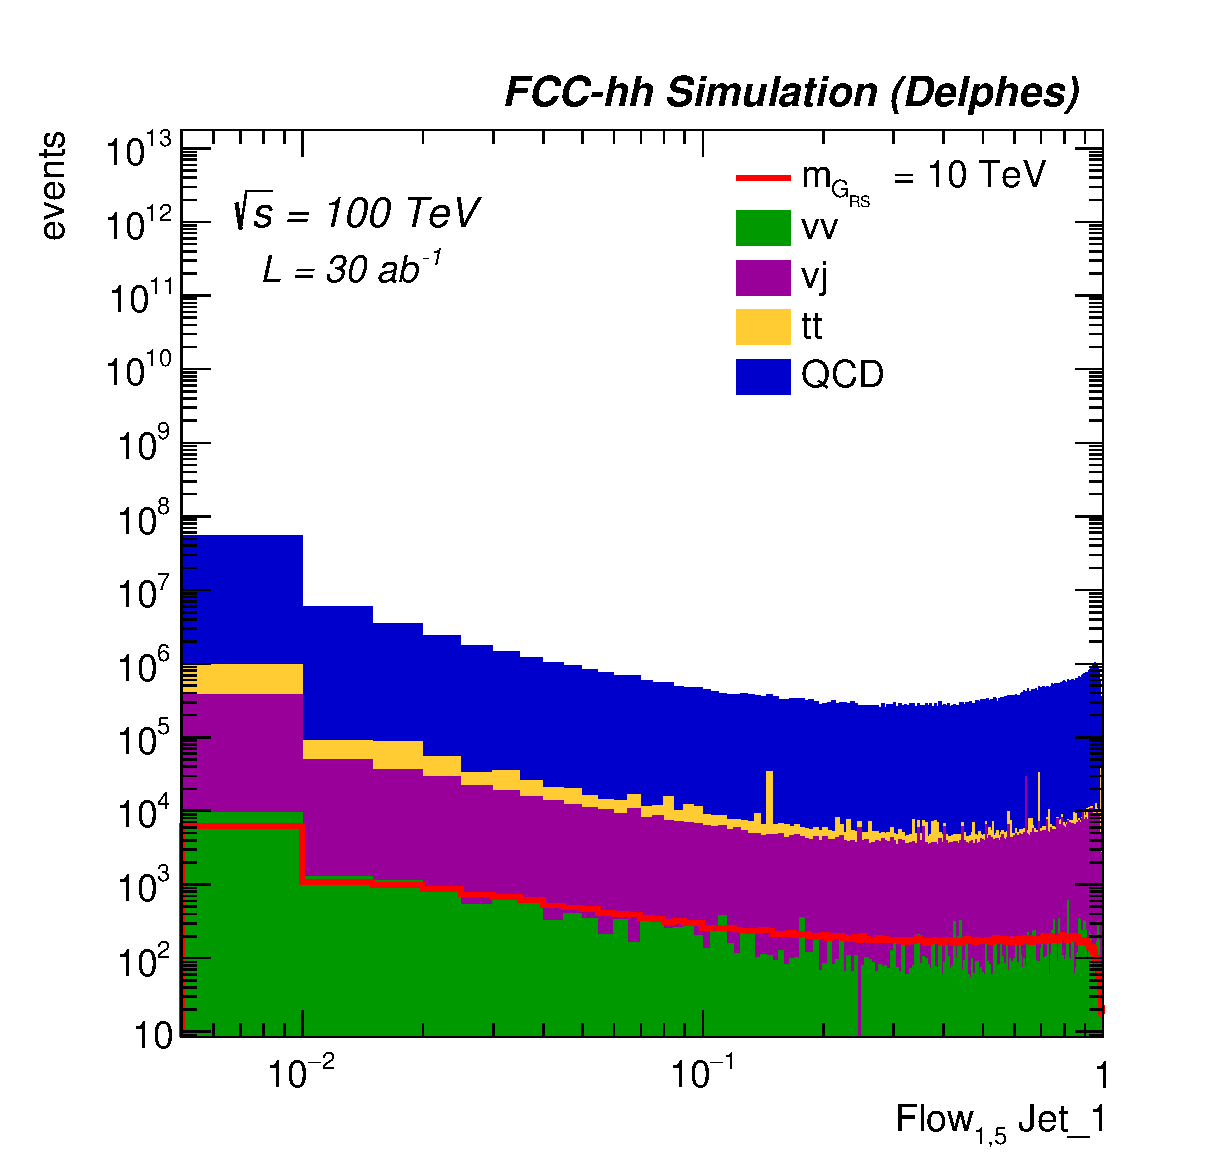
\includegraphics[width=0.45\textwidth]{Fig/TMVA/Jet1_Flow15_sel0_nostack_logx.eps}
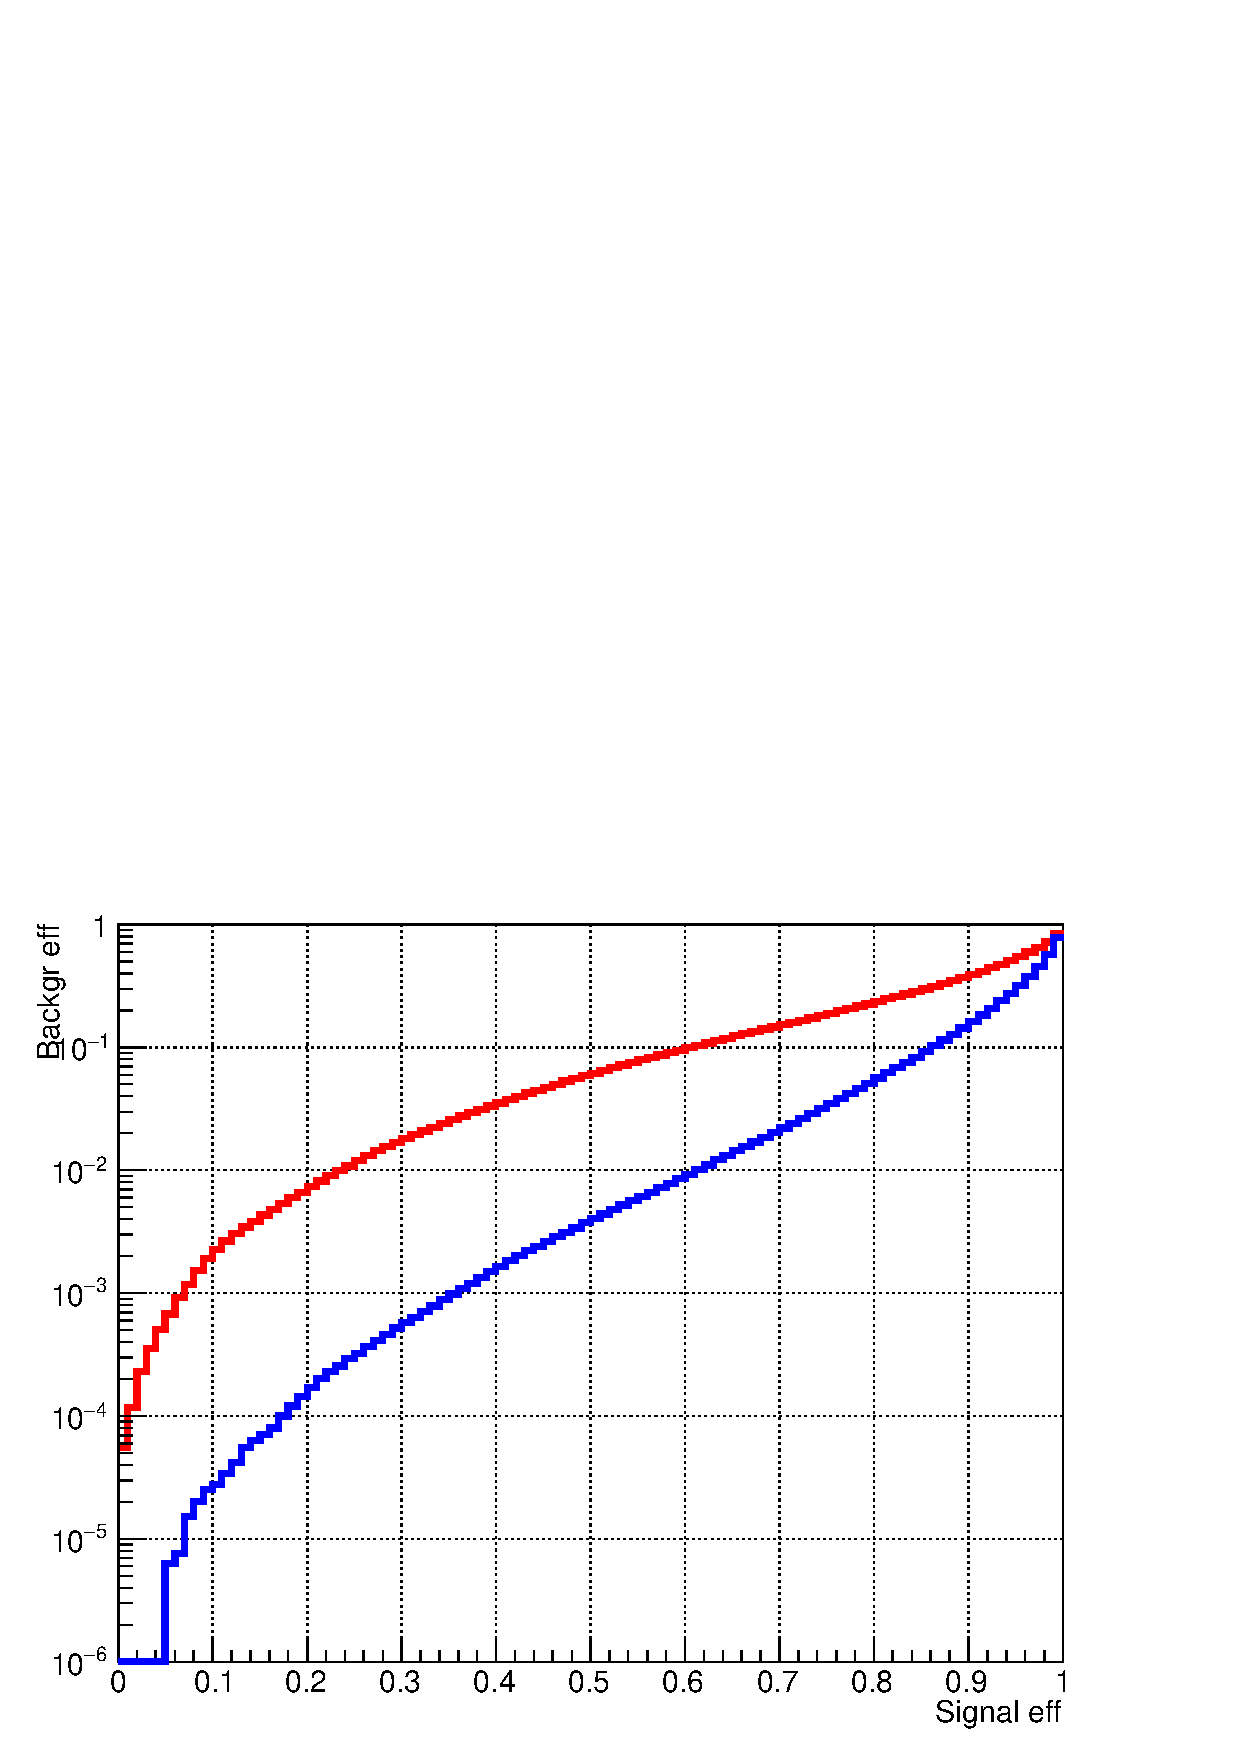
\includegraphics[width=0.45\textwidth,trim={0 0.5cm 0 0},clip]{Fig/TMVA/effQCD_vs_effWhadBlue_thadRed_log.pdf}
\caption{Left: Energy-flow ($E_{F}(1,0.05)$) observable for W and QCD jets. Right: Light jet rejection versus tagging efficiency for the $W$ tagger (blue) and top tagger (red).}
\label{fig:TMVA_final_result}
\end{figure}

%\clearpage
%\newpage

%%%%%%%%%%%%%%%%%%%%%%%%%%%%%%%%%%%%%%%%%%%%%%%%%%%%%
\subsection{Tag Rate Function}
\label{subsec:trf}
The modeling of the backgrounds in the high tagging regimes is a challenging task.
The requirement of $b$ tagging in some MC samples can drastically reduce the available statistics.
This shortage of events that pass the $b$-tagging cut in the signal regime, in conjunction with the large cross section of some of the backgrounds can lead to very spiky templates.
\newline
To overcome this problem the tag rate function (TRF) method is introduced.
By using the TRF method, no event is cut based on its $b$-tagging count, but instead all the events are weighted.
This weight can be interpreted as the probability of the given event to contain the desired number of $b$ jets.
To achieve this, the tagging efficiency (a function of $\eta$, $\pt$ and true jet flavour) was
used to calculate the event weight based on the kinematics and flavour of the jets found in each event.
\newline
Given a jet with $\eta$, $\pt$ and flavour $f$, its tagging probability can be noted as:
\begin{equation*}
	\varepsilon \left(f,|\eta|,\pt\right)
\end{equation*}
\newline
For a given event with $N$ jets, its probability of containing exactly one $b$-tag jet can be computed as:
\begin{equation*}
	P_{=1} = \sum\limits_{i=1}^N \left( \varepsilon_{i} \prod\limits_{i \neq j} \left( 1 - \varepsilon_{j} \right) \right)
\end{equation*}
\newline
In the same way, it can be used to compute the probability for inclusive $b$-tag selections:
\begin{align*}
	P_{=0} &= \prod\limits_{i=1}^N \left( 1 - \varepsilon_{j} \right) \\
	P_{\geq 1} &= 1 - P_{=0}
\end{align*}
\newline
It was verify that the TRF methods agrees well with the direct tagging.

%%%%%%%%%%%%%%%%%%%%%%%%%%%%%%%%%%%%%%%%%%%%%%%%%%%%%
\subsection{Mass spectrum fit}
Despite the fact that very large amount of Monte-Carlo statistic has been simulated in bins of $\hht$
and the usage of techniques to save events with TRF methods,
there are still large statistical fluctuations from high weight events.
In order to reduce this effect, a function is used to fit the background distribution,
\begin{equation}
f(z)=p_1(1-z)^{p_2}z^{p_3}z^{p_{4}logz}
\end{equation}
where $z=m_{jj}/\sqrt{s}$. This fit is used in order to have a smooth shape for the backgrounds, while the normalisation is taken prior to the fit (see figure~\ref{fig:hadronicresonances_nofit}).

\begin{figure}[!htb]\centering
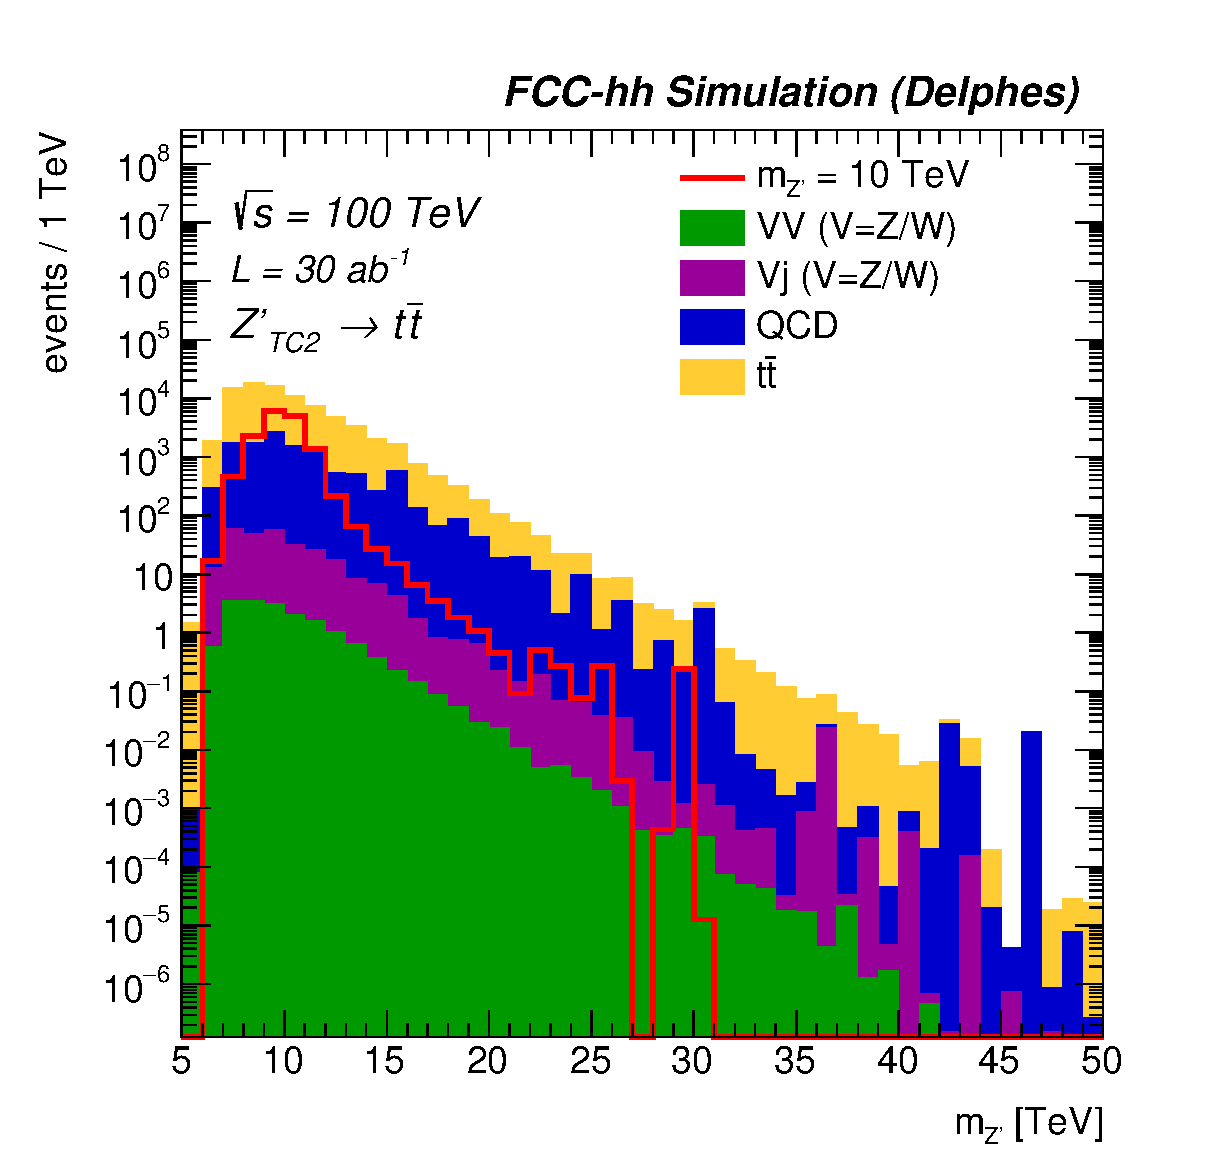
\includegraphics[width=0.45\columnwidth]{Fig/Zptt/Mj1j2_pf08_MetCorr_sel8_nostack_log.eps}
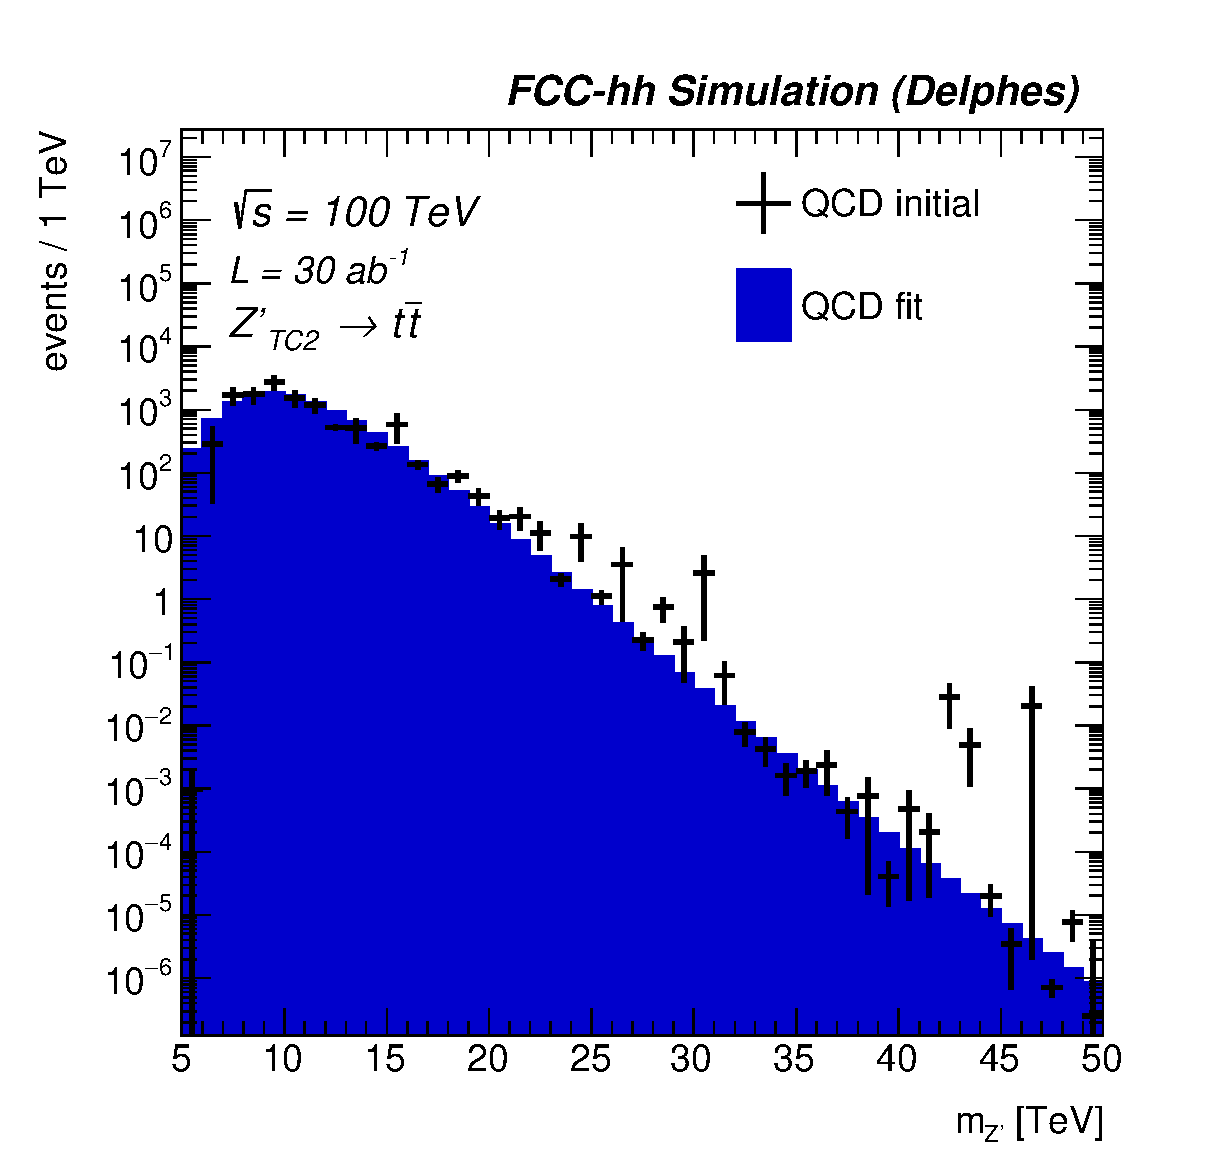
\includegraphics[width=0.45\columnwidth]{Fig/Zptt/Zptt_QCD_sel8_Mj1j2_pf08_MetCorr_fit.eps}
\caption{Invariant mass prior to fit.}
\label{fig:hadronicresonances_nofit}
\end{figure}


\section{Di-lepton channels}
\label{sec:lep}

\subsection{The \ee\ final state}
\label{sec:lepee}

\subsection{The \mumu\ final state}
\label{sec:lepmumu}

\subsection{The \tautau\ final state}
\label{sec:leptautau}

\section{Hadronic final states}
\label{sec:hadronic}

\subsection{Introduction}
\label{sec:hadintro}

\subsection{The \jj\ final state}
\label{sec:hadjj}

\subsection{The \ttbar\ final state}
\label{sec:hadtt}

\subsection{The \ww\ final state}
\label{sec:hadww}

\section{Characterisation of a Z' discovery}
\label{sec:zprimedisc}

  \label{sec:zprimeflav}

\section{Conclusion}
\label{sec:conc}


\appendix
\section{Some title}
Please always give a title also for appendices.





\acknowledgments

This is the most common positions for acknowledgments. A macro is
available to maintain the same layout and spelling of the heading.

\paragraph{Note added.} This is also a good position for notes added
after the paper has been written.





% The bibliography will probably be heavily edited during typesetting.
% We'll parse it and, using the arxiv number or the journal data, will
% query inspire, trying to verify the data (this will probalby spot
% eventual typos) and retrive the document DOI and eventual errata.
% We however suggest to always provide author, title and journal data:
% in short all the informations that clearly identify a document.

\bibliographystyle{JHEP}
\bibliography{refs}

% Please avoid comments such as "For a review'', "For some examples",
% "and references therein" or move them in the text. In general,
% please leave only references in the bibliography and move all
% accessory text in footnotes.

% Also, please have only one work for each \bibitem.


\end{document}
